\chapter{Experimental setup}
This chapter provides a description of the experimental setup used to evaluate the clustering aggregation protocol in different quantum computing environments, both on a simulator and on real hardware. The protocol was tested on three distinct platforms: a simulator for a neutral-atom quantum computer, specifically the Pulser simulator by PASQAL; the Fresnel neutral-atom quantum computer, also developed by PASQAL; the Advantage quantum annealer with Pegasus topology, developed by D-Wave.

% aggiungere descrizione macchine 
\section{Quantum platforms}
\subsection{Programmable neutral-atom arrays}

\subsection{QuTiP}
The Quantum Toolbox in Python, also known as QuTiP, is an object oriented Python framework designed to represent and simulate the dynamics of open and closed quantum systems \cite{Johansson2012}. 

The core of information representation in QuTiP is the \texttt{Qobj} class, which is used to represent both quantum states (such as pure states or density matrices) and quantum operators (such as Hamiltonians or measurement operators). The \texttt{Qobj} class offers methods to perform matrix operations like addition, multiplication and tensor product, which are essential to manipulate quantum systems; sparse matrix encoding of objects allows these operations to be executed relatively efficiently.

To perform simulations using QuTiP, it is necessary to specify the initial conditions of the system, for example ket vectors or density matrices, and a Hamiltonian or other operators, which describe the time evolution and possible dissipations. It is then possible to select different kinds of solvers, such as the Monte Carlo wave function method for a Schrödinger equation describing evolution of pure states, or a numerical approach for a Lindblad master equation in the case of open systems.

Results are presented in the form of evolved states at fixed intervals throughout the simulation time windows. Additionally, QuTiP allows to perform the calculations of expectation values for observables (such as spin, position, or energy) over time.

Since QuTiP does not directly support neutral-atom systems, Pulser contains a library that acts as an interface to QuTiP, in order to simplify the definition of neutral-atom arrays and the simulation of experiments with laser pulses. 

\section{Dataset}
\label{sec:dataset}
The dataset used to test the protocol is shown in figure \ref{fig:dataset}. It was first introduced by Gionis, Mannila and Tsaparas to test classical clustering aggregation algorithms \cite{dataset}; it was then used by Li and Latecki to test a clustering aggregation protocol that uses simulated annealing \cite{aggregation}.

It is specifically designed to contain different shapes and configuration of points, in such a way that most clustering algorithms fail to produce a correct clustering. It is made up of 7 clusters and 788 points in total.

\begin{figure}[ht!]
  \centering 
  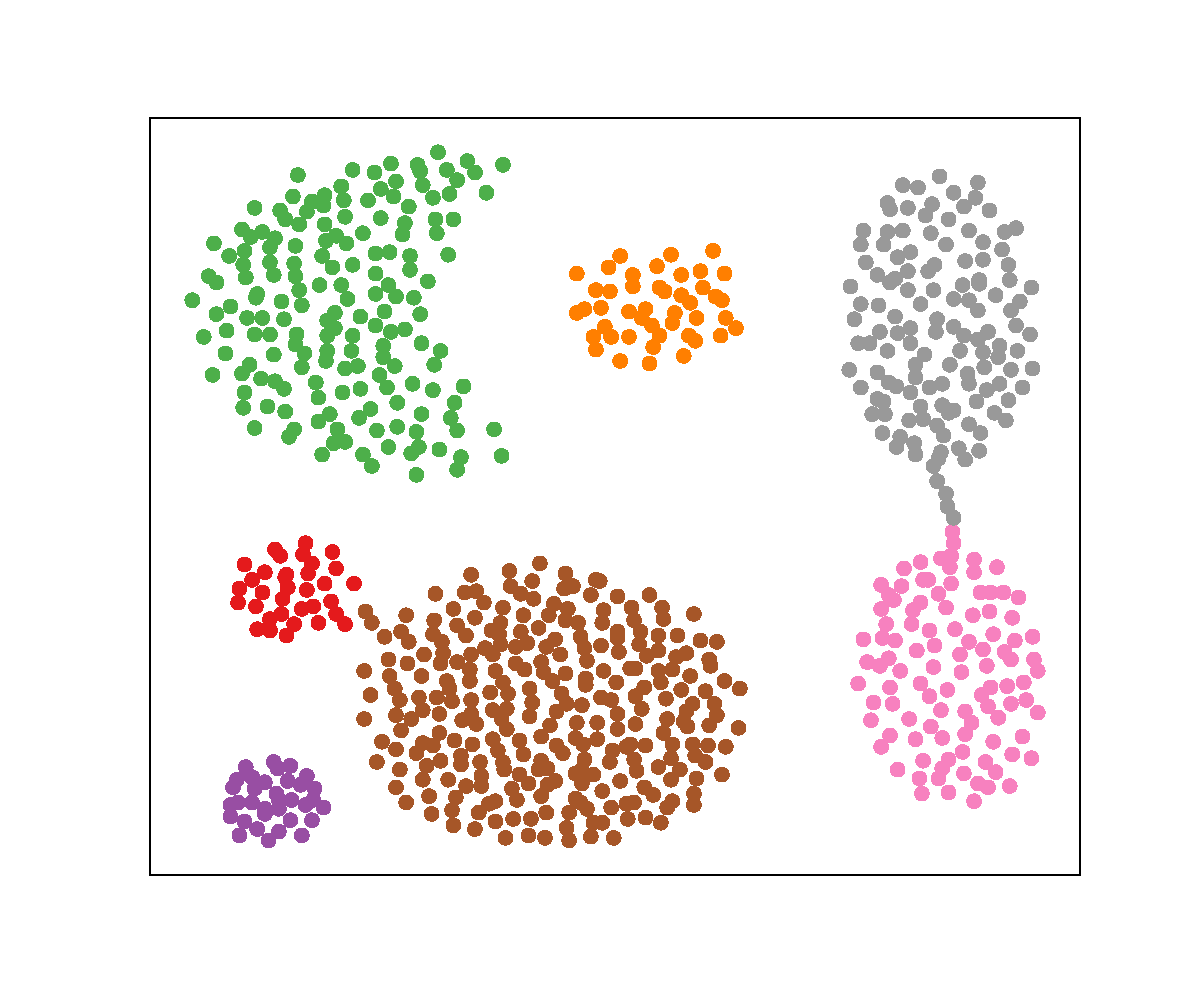
\includegraphics[width=0.72\textwidth]{figures/05experimental_setup/dataset.pdf}
  \caption{Dataset plot}
  \label{fig:dataset}
\end{figure}

\section{Evaluation metrics}
Different metrics were used to evaluate the quality of single clusters and of clustering algorithms as a whole. Silhouette score was used as a factor to weigh clusters in the clustering aggregation protocol; Rand index was used to compare the overall quality of the clustering algorithms and aggregation protocols. % aggiungere anche intersezione insiemistica? 

\subsection{Silhouette score}
The silhouette score is a metric used to evaluate clustering quality, introduced by Rousseeuw \cite{Rousseeuw1987}. The score is computed for each point in the dataset and reflects both its cohesion with points in the same cluster, as well as the separation with respect to points in different clusters. Specifically, the silhouette score of a point $p$ in the dataset is defined as 
\begin{equation}
  \label{eqn:silhouette}
  S_{p} = \frac{b_{p} - a_{p}}{\max({a_{p}, b_{p}})},
\end{equation}
where $a_{i}$ is the average distance from the point to other points in the same cluster (intra-cluster distance), and $b_{i}$ is the average distance to points in the nearest different cluster (inter-cluster distance). The score ranges between -1 and 1, where values close to 1 indicate that points are well-clustered, with high cohesion and good separation, while negative values suggest points may have been assigned to the wrong cluster. 

A quantification of the quality for a single cluster can be obtained by computing the average of the silhouette score of the point it contains; more formally, for a cluster $c_{i}$, the formula for its average silhouette ($AS_{i}$) is 
\begin{equation}
  \label{eqn:cluster_silhouette}
  AS_{i} = \frac{\sum_{p \in c_{i}} S_{p}}{|c_{i}|}.
\end{equation}

\subsection{Rand index}
The Rand index is a metric that quantifies the similarity between two data clusterings, first proposed by Rand \cite{Rand1971}. It is computed by considering all possible pairs of points in the dataset and assessing whether they are assigned to the same or different clusters in the two clusterings being compared. The index assumes values between 0 and 1, with 1 indicating perfect agreement between the two clusterings. 

Given two clusterings $\mathcal{C}_{1}$ and $\mathcal{C}_{2}$, their Rand index is computed as  
\begin{equation}
  \label{eqn:rand}
  RI = \frac{a + b}{a + b + c + d},
\end{equation}
where
\begin{itemize}
  \item $a$ is the number of point pairs that are put in the same cluster in both clusterings;
  \item $b$ is the number of point pairs that are put in different clusters in both clusterings; 
  \item $c$ is the number of point pairs that are put in the same cluster in $\mathcal{C}_{1}$, but in different clusters in $\mathcal{C}_{2}$;
  \item $d$ is the number of point pairs that are put in different clusters in $\mathcal{C}_{1}$, but in the same cluster in $\mathcal{C}_{2}$.
\end{itemize}

\section{Description of experiments}

\subsection{Pulser experiment}
The Pulser neutral-atom computer simulator was used to test the aggregation protocol on the dataset discussed in \ref{sec:dataset}; 

Two different clustering algorithms were run on the dataset, DBSCAN and Spectral Clustering. Hyperparameters were tuned empirically, in order to ensure an overall amount of clusters inferior or equal to 14, so as not to exceed the amount of qubits the simulator can handle \cite{Johansson2012}.

\begin{figure}
  \centering 
  
\end{figure}